\documentclass[a4paper,12pt]{report}

\usepackage{alltt, fancyvrb, url}
\usepackage{graphicx}
\usepackage[utf8]{inputenc}
\usepackage{hyperref}
\usepackage{float}

\usepackage[italian]{babel}

\usepackage[italian]{cleveref}

\title{A.A. 2020/2021\\Relazione di progetto\\Programmazione di reti}

\author{Leon Baiocchi 0000938801, Federico Brunelli 0000934810}
\date{\today}

\begin{document}

\maketitle

\begin{abstract}
Questo documento è una relazione del progetto d'esame di Programmazione di Reti, in particolare della \textbf{TRACCIA 1 - Progetto IoT}.
%
Lo scopo di questo documento è quello di permettere la comprensione dei dettagli di progettazione e del funzionamento del seguente progetto.
%
Inoltre, dovrebbe permettere un'ampia visione del lavoro svolto dal team, che ricordiamo essere composto da Leon Baiocchi e Federico Brunelli, in termini di organizzazione, oltre che di progettazione.
%
Per ciascuna delle sezioni del documento sarà fornita una descrizione di ciò che riguarda ognuna di esse, a partire da quella inerente alla fase di \emph{Analisi} fino ai \emph{Commenti finali} per poi arrivare ad una piccola appendice munita di \emph{Guida utente}, utile se si volesse mettere in azione l'applicativo.

Riferirsi all'\emph{Indice} presente nella pagina sottostante per maggiori informazioni.
%
Buona lettura!
\end{abstract}

\tableofcontents

\chapter{Analisi}

Il Fondo Ambiente Italiano ci ha commissionato un progetto per la salvaguardia dell'ambiente.
%
Lo scopo di questo progetto consiste nella raccolta di misurazioni relative a temperatura e umidità del terreno in una zona a rischio.
%
La fondazione ha messo a disposizione quattro dispositivi per il rilevamento dati, denominati Smart Meter IoT, e un Gateway per instradare le misurazioni raccolte dai vari device verso un server cloud centrale di proprietà del FAI.
%
La rete che permette ai device di scambiare dati con il gateway ha un'indirizzamento di \emph{Classe C} del tipo \textbf{192.168.1.0/24}.

Essa non è l'unica in quanto vi è un'altra rete, che permette al gateway di inoltrare messaggi al \emph{Cloud Server} del FAI tramite un'indirizzamento di classe \textbf{10.10.10.0/24}.

I quattro dispositivi si occupano di inviare, una volta al giorno, i dati raccolti attraverso una connessione UDP verso il gateway, il quale, dopo aver ricevuto tutti i pacchetti, inoltrerà tali dati al cloud tramite una connessione TCP.

Essendo questa una relazione di progetto del corso di Programmazione di reti, ci concentreremo solo sugli aspetti di rete, escludendo quelli di IoT.
\newline
\newline
\newline
\begin{figure}
\centering{}
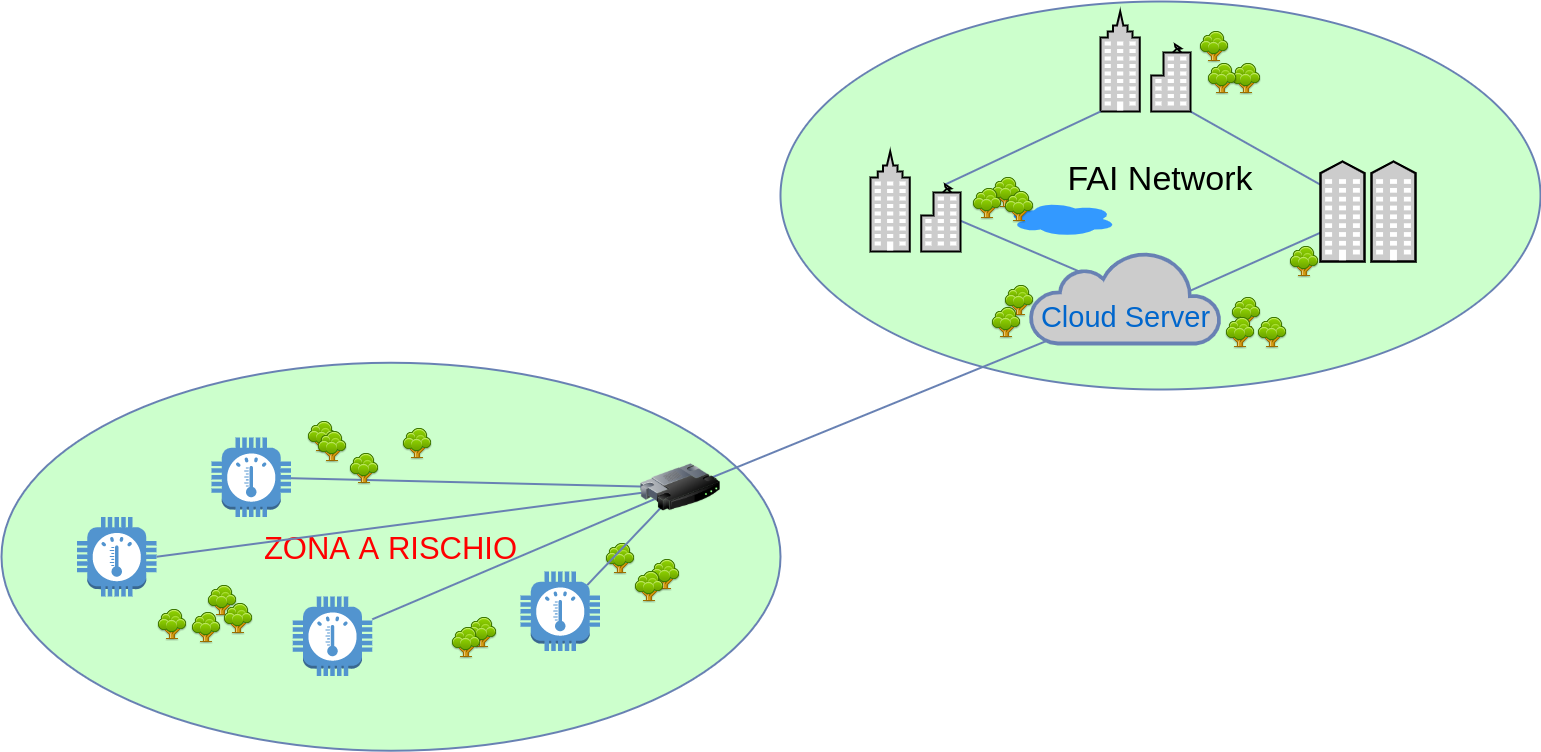
\includegraphics[width=\textwidth, height=15em]{img/Scenario.png}
\caption{Scenario}
\label{img:analysis}
\end{figure}

\section{Requisiti}

Il software, commissionato dal FAI, consiste nel realizzare un \emph{network} che permetta ai quattro \textbf{dispositivi} di interfacciarsi con il \textbf{gateway}.
%
Quest'ultimo possiede un'ulteriore interfaccia di rete, quindi il cloud è in un'altro \emph{network}, che permette la comunicazione con il \textbf{server cloud}.

\subsection*{Requisiti funzionali}
\begin{itemize}
	\item \textbf{Addressing}: i \emph{dispositivi} situati nella zona a rischio e l'\emph{interfaccia di rete del gateway} adibita alla ricezione delle misurazioni devono avere \underline{indirizzi IP} appartenenti alla classe \textbf{192.168.1.0/24} mentre l'interfaccia del gateway che si occupa di instradare le misurazioni dei device verso il \emph{server cloud} e quest'ultimo devono avere \underline{indirizzi IP} del tipo \textbf{10.10.10.0/24}.
	\item I quattro \emph{dispositivi} devono salvare su un \textbf{file} le misurazioni ottenute indicando \emph{ora della misurazione, valore della temperatura} e \emph{valore dell'umidità}.
	%
	I quattro dispositivi si occupano di inviare, \emph{una volta al giorno}, i dati raccolti attraverso una connessione UDP verso il gateway.
	\item Il \emph{gateway} deve ricevere i dati delle misurazioni dai \emph{dispositivi} e instradarli verso il \emph{cloud}.
	\item E' inoltre richiesto che il \emph{server cloud} visualizzi, su una console, le misurazioni ottenute nel seguente formato:
	\newline
    \textbf{IpAddressDevice1–OraMisura–ValoreTemperatura–ValoreUmidità}
\end{itemize}

\subsection*{Requisiti non funzionali}
\begin{itemize}
	\item E' importante che i \emph{dati} vengano scambiati in maniera efficace e consistente riducendo al minimo il sovraccarico dei vari \emph{canali di trasmissione}.
	\item E' previsto anche che siano prese delle misurazioni riguardanti i \emph{\underline{tempi di trasmissione}} di ciascun \textbf{canale}
\end{itemize}

\section{Analisi e modello del dominio}

La scenario è il seguente: abbiamo a disposizione \textbf{4 dispositivi IoT} in grado di ottenere \emph{dati} dalle misurazioni di temperatura e umidità. 
%
Essi si trovano all'interno di una \textbf{zona a rischio} e si interfacciano con un \textbf{gateway} al quale inviano \textbf{periodicamente} i dati raccolti attraverso il \underline{protocollo UDP}.

Dall'altra parte invece, il \textbf{cloud server} centrale situato all'interno della \emph{rete} del FAI aspetta che il gateway si connetta tramite \underline{connessione TCP} ed inizia a ricevere i dati delle misurazioni, che possono arrivare già formattati correttamente oppure ancora da formattare.

Essenziale il compito del \emph{gateway} che deve ricevere i dati in arrivo dai \textbf{dispositivi} per poi riuscire ad instradarli in maniera efficente, eventualmente formattandoli correttamente.
%
La \emph{dimensione dei canali trasmissivi} potrebbe dipendere dal momento in cui si formattano le misurazioni.

Da notare, inoltre, come gli host siano distribuiti su due reti diverse, una situata nella \emph{zona a rischio} mentre l'altra è la \emph{rete del FAI}.
%
Per questo motivo gli host delle due reti hanno \textbf{indirizzamento} diverso. 

Una visione in UML di come comunicano tra di loro gli host è osservabile nella \Cref{img:analysis}.
\newline
\newline
\begin{figure}
\centering{}
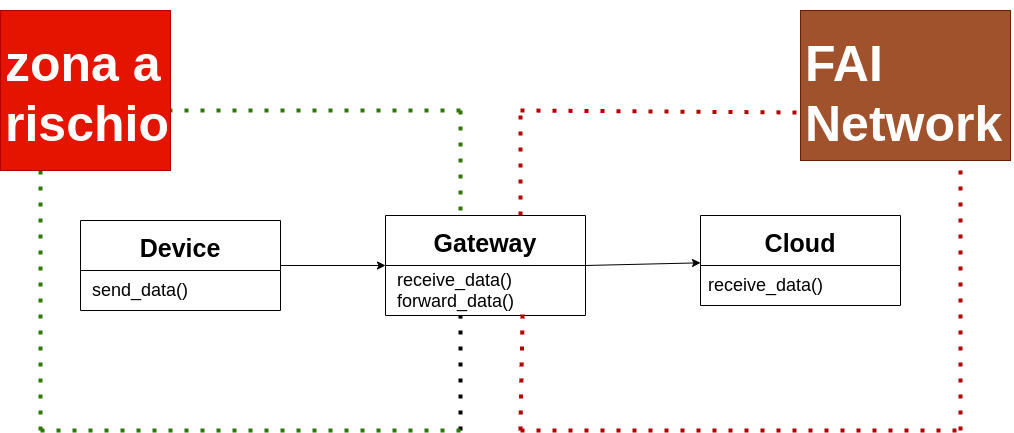
\includegraphics[width=\textwidth, height=15em]{img/AnalysisUML.png}
\caption{Schema UML delle comunicazioni tra gli host}
\label{img:analysis}
\end{figure}

\chapter{Design}
Come già detto nel capitolo precedente, ci occuperemo principalmente degli aspetti di rete, \emph{emulando} le funzionalità dei quattro dispositivi IoT.
%
Inoltre, data la natura didattica del progetto, il sistema deve utilizzare l'interfaccia di loopback per simulare le varie connessioni tra i differenti \textbf{hosts} e perciò l'\textbf{IP address} e il \textbf{MAC address} sono impostati con un valore di \emph{default}.

Per modellare al meglio le varie entità abbiamo preferito sfruttare la \emph{programmazione ad oggetti}.
%
Questo per garantire una maggior leggibilità del codice oltre che una maggiore facilità di manutenzione dello stesso.

\section{Architettura}

Il sistema presenta due \textbf{network} differenti, quello della zona a rischio e quello del FAI.

Il committente ha richiesto che le classi di indirizzamento delle due reti siano di tipo C e figurino nel seguente modo: \textbf{192.168.1.0/24} e \textbf{10.10.10.0/24}. 
%
Entrambe hanno quindi stessa \emph{maschera di sottorete}: \emph{255.255.255.0}, che permette di indirizzare 255 possibili host, se, oltre ai già 254 indirizzi disponibili, viene solo considerato l'indirizzo del default gateway e non quello di broadcast.

\emph{Perchè lo consideriamo come indirizzo valido?}

Perchè avendo un dispositivo che deve avere funzione di \emph{router} come il nostro \textbf{Gateway} l'indirizzo del \underline{default gateway} fa proprio al caso nostro dato che l'host da contattare per mandare messaggi da una rete all'altra è proprio quello.
%
Motivo per il quale questo particolare dispositivo ha \underline{due} interfaccie di rete.
\newline
\newline
\newline
Gli indirizzi assegnati ai vari hosts delle due reti sono:
\begin{itemize}
    \item \textbf{\underline{Zona a rischio}}
    \begin{itemize}
        \item \emph{\textbf{Device\_1}}: 
        \begin{itemize}
            \item IP: 192.168.1.10
            \item MAC: 36:DF:28:FC:D1:67
        \end{itemize}
        \item \emph{\textbf{Device\_2}}: 
        \begin{itemize}
            \item IP: 192.168.1.15
            \item MAC: 04:EA:56:E2:2D:63
        \end{itemize}
        \item \emph{\textbf{Device\_3}}: 
        \begin{itemize}
            \item IP: 192.168.1.20
            \item MAC: 6A:6C:39:F0:66:7A
        \end{itemize}
        \item \emph{\textbf{Device\_4}}: 
        \begin{itemize}
            \item IP: 192.168.1.25
            \item MAC: 96:34:75:51:CC:73
        \end{itemize}
        \item \emph{\textbf{Gateway}}: 
        \begin{itemize}
            \item IP: 192.168.1.1
            \item MAC: 7A:D8:DD:50:8B:42
        \end{itemize}
    \end{itemize}
    \item \textbf{\underline{FAI network}}
    \begin{itemize}
        \item \emph{\textbf{Gateway}}: 
        \begin{itemize}
            \item IP: 10.10.10.1
            \item MAC: 7A:D8:DD:50:8B:42
        \end{itemize}
        \item \emph{\textbf{Cloud server}}: 
        \begin{itemize}
            \item IP: 10.10.10.2
            \item MAC: FE:D7:0B:E6:43:C5
        \end{itemize}
    \end{itemize}
\end{itemize}

Gli \textbf{indirizzi MAC} impostati per ogni interfaccia di rete sono tutti \emph{locally administered}(U/L bit = 1) e \emph{unicast}(I/G bit = 0).
%
Per una visione ampia e abbastanza dettagliata dell'architettura di rete e delle funzioni che i vari host svolgono all'interno di essa è necessario prestare attenzione alla \Cref{img:howhostscommunicate}
\begin{figure}[H]
\centering{}
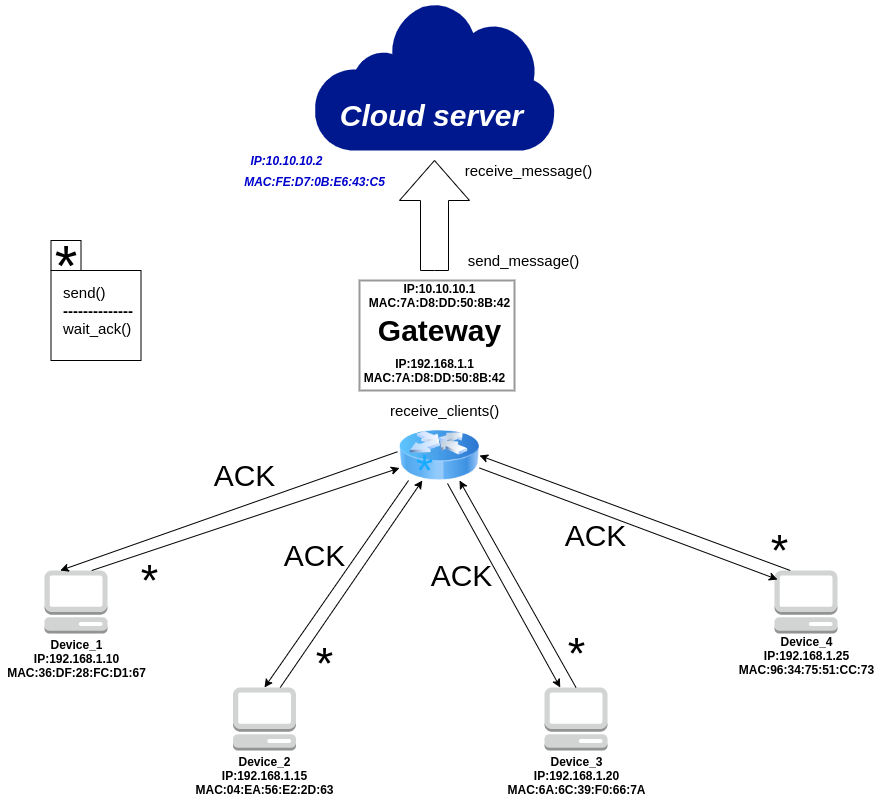
\includegraphics[width=\textwidth, height=30em]{img/HowHostsCommunicate.png}
\caption{Schema rappresentativo dell'architettura di rete e delle operazioni di base svolte dai relativi dispositivi}
\label{img:howhostscommunicate}
\end{figure}
%
\section{Design dettagliato}

In questa sezione approfondiremo alcuni elementi del design con maggior dettaglio.
Analizziamo quindi la \cref{img:howhostscommunicate}: partendo dal modo in cui i \textbf{device} comunicano con il \textbf{gateway}(parte bassa dello schema), durante la fase di progettazione siamo giunti alla conclusione che, essendo UDP un protocollo di trasporto non garante di \emph{data reliability}, avremmo dovuto implementare da soli un meccanismo di avvenuta ricezione del pacchetto.

Questo meccanismo, già noto, sfrutta i messaggi \textbf{ACK}nowledged per garantire una corretta fruizione dei \emph{pacchetti di rete} ed assicurarne la ricezione.
E' un sistema molto simile, e soprattutto ispirato, al meccanismo utilizzato dal protocollo \emph{TCP}.
%
In questo modo i dispositivi possono sapere se il pacchetto inviato è stato consegnato a destinazione.

\begin{figure}[H]
\centering{}
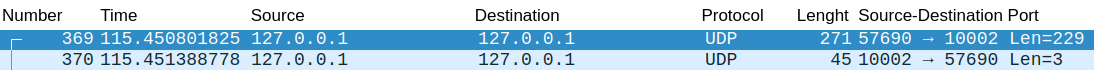
\includegraphics[width=\textwidth,height=25]{img/dev1_send.png}
\caption{Cattura Wireshark: comunicazione tra \emph{device} e \emph{gateway}}
\label{img:devsend}
\end{figure}
Una volta che il \emph{gateway} ha inoltrato l'ACK, salva il pacchetto arrivato in una \textbf{arp table modificata}, nel senso che oltre a tenere memoria di ogni coppia indirizzo IP, indirizzo MAC; memorizza per ognuna di esse l'ultimo pacchetto ricevuto dal device con IP corrispondente.
%
Ad ogni ricezione viene poi verificato se tutti e 4 i device hanno inviato i dati e se ciò è vero tutti i payload vengono prima formattati e inseriti all'interno di un unico grande pacchetto che successivamente, inseriti gli \textbf{headers}, viene inoltrato al \emph{cloud} il quale riceve e stampa a video tutte le misurazioni nel formato richiesto. Proseguiamo ora con una descrizione ancora più nel dettaglio di tutti i vari componenti.

\begin{figure}[H]
\centering{}
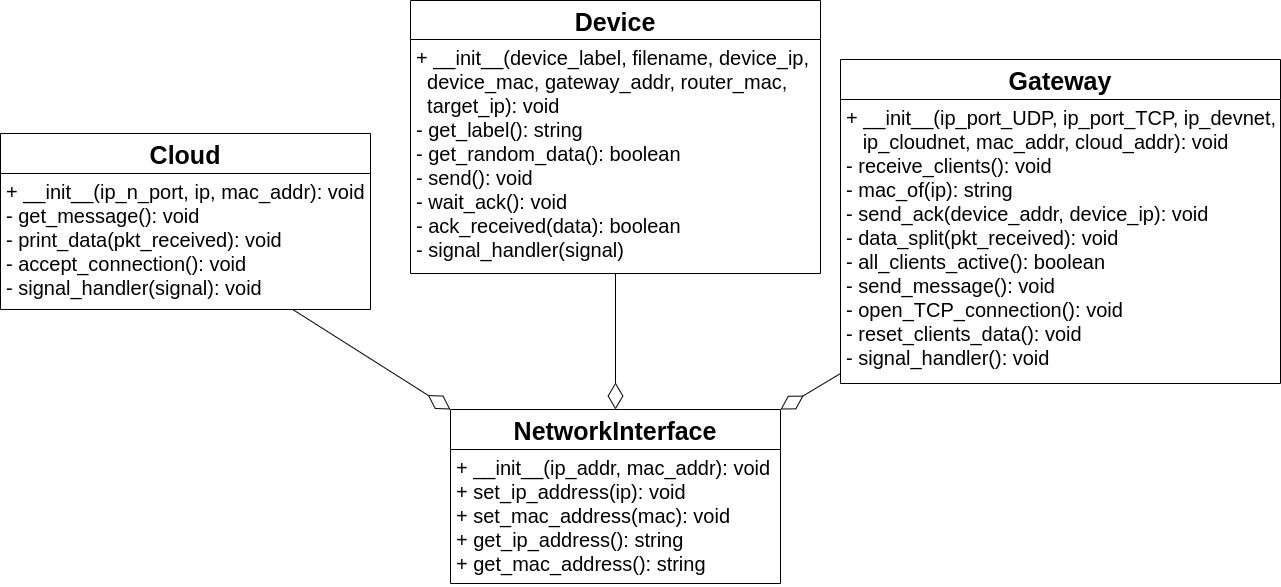
\includegraphics[width=\textwidth,height=20em]{img/UML_Hosts_Classes.png}
\caption{UML figurativo delle classi relative agli host}
\label{img:uml_hosts_classes}
\end{figure}
Per rendere più chiaro il network, abbiamo preferito distinguere le interfacce dei vari host, così da permettere una maggiore leggibilità.
Va sottolineato il fatto che il \textbf{Gateway} possiede due interfacce di rete:
\begin{itemize}
    \item \emph{device\_interface}
    \item \emph{cloud\_interface}
\end{itemize}
La prima permette la comunicazione con i device, mentre la seconda si interfaccia con il server centrale.
Come si può osservare nella \Cref{img:uml_hosts_classes}, la classe \textbf{NetworkInterface} tiene traccia dell'indirizzo mac dell'host di riferimento e l'indirizzo IP legato alla rete.
\begin{figure}[H]
\centering{}
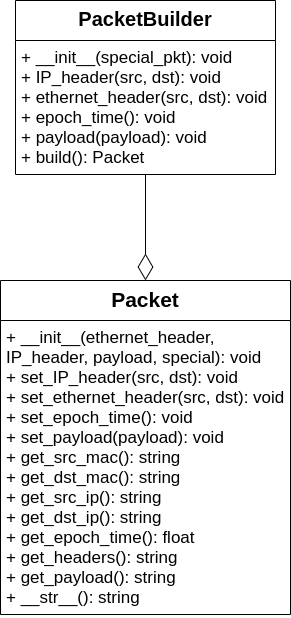
\includegraphics[width=13em,height=30em]{img/UML_Packet_PacketBuilder.png}
\caption{UML figurativo del pacchetto trasmesso}
\label{img:uml_packet_packetbuilder}
\end{figure}
%
Questo schema rappresenta la classe \textbf{Packet}: astrazione del pacchetto di rete che viene trasmesso tra i vari host. Esso contiene l'intestazione riguardante gli \emph{indirizzi} \textbf{MAC} e \textbf{IP} del \textbf{mittente} e del \textbf{destinatario} e l'\textbf{epoch time} relativo all'inoltro del messaggio, utile se si vuole calcolare per esempio il \emph{tempo impiegato} per la \emph{trasmissione} di tale pacchetto, proprio come nel nostro caso. Inoltre, nel pacchetto vi `e presente il messaggio vero e proprio(\textbf{payload}).

Un oggetto \emph{Packet} è istanziabile attraverso il costruttore che permette anche di specificare se si tratta di un \textbf{"pacchetto speciale"} come potrebbe essere nel caso di un \emph{ACK}. 
%
Ma non solo, difatti abbiamo pensato che potesse tornare utile la creazione a cascata di un oggetto simile in modo da permettere di creare una molteplicità di pacchetti differenti facilmente.
%
E' per questo che abbiamo sfruttato il pattern \textbf{builder} dando vita così alla classe PacketBuilder la quale fornisce metodi a cascata per la creazione degli \emph{headers} ed il \emph{payload}, infine vi è il metodo build() che mette insieme i componenti generando un'oggetto Packet del tipo definito.

Tornando alla classe Packet è da delineare il fatto che i \emph{parametri} del costruttore siano \textbf{opzionali}, questo poichè abbiamo voluto dare spazio a varie interpretazioni della classe, difatti con tali argomenti è possibile per esempio creare dapprima un pacchetto vuoto per poi aggiungere "strada facendo" i vari elementi(headers e payload).
%
Sono poi presenti tutti i rispettivi getters di headers, sub-headers(quali sorgente e destinazione di IP header e l'ethernet header) e payload.

Viene fornito anche un metodo per \emph{convertire} il contenuto del pacchetto in stringa.

\subsection{Classi host: Device}

\begin{figure}[H]
\centering{}
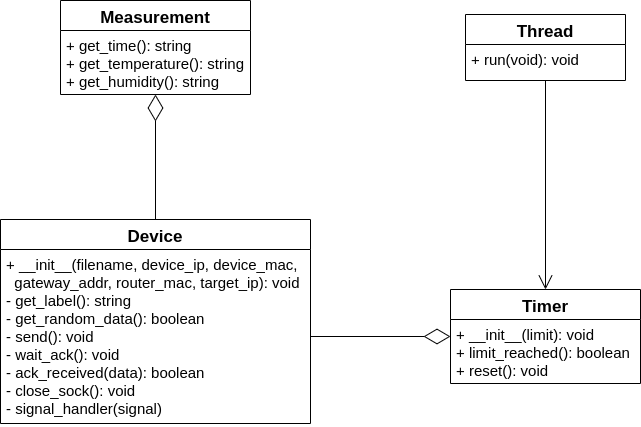
\includegraphics[width=\textwidth,height=23em]{img/UML_Device_Timer.png}
\caption{UML rappresentativo della classe Device}
\label{img:uml_device_timer}
\end{figure}

In figura viene mostrata la struttura della classe \textbf{Device} che rappresenta un dispositivo IoT, essa si compone di oggetti di altre classi: \textbf{Measurement}, che consente di ottenere misurazioni randomiche; \textbf{Timer}, classe figlia di \emph{Thread} che si occupa di scandire il tempo tra l'invio di un pacchetto e un altro.

\textbf{Device} presenta un costruttore, dove avviene tutto, con \emph{parametri obbligatori} ed una serie di metodi tutti privati.
%
Abbiamo fatto questa scelta per \underline{tutte} le classi che rappresentano dispositivi di rete perchè volevamo rappresentare degli \emph{host specifici} per questo progetto e non universali, per cui ci siamo orientati verso un maggior incapsulamento delle informazioni.

Prima di partire a descrivere il funzionamento della classe \emph{Device} è opportuno introdurre prima le altre due classi:
%
\begin{itemize}
\item \emph{Measurement} è costituita da 3 metodi pubblici che ritornano rispettivamente un'\textbf{orario}, un valore di \textbf{temperatura} scelto tra un range di valori prestabiliti, un valore indicante l'\textbf{umidità} anch'esso scelto allo stesso modo. Il tipo di questi 3 valori di ritorno è sempre lo stesso: una \emph{stringa}.

\item \emph{Timer} è una sotto-classe di \emph{Thread} per cui ne eredita le caratteristiche, aggiungendone altre: questa classe difatti è essenziale per inviare \underline{\emph{periodicamente}} messaggi al \emph{gateway}. Un'oggetto di questo tipo ha infatti un timer interno ed un limite, da impostare via costruttore. Quando il timer giunge al limite il metodo \emph{limit\_reached()} ritorna \emph{True}, dopodichè va fatta la \emph{reset()} del timer se si vuole continuare ad utilizzarlo.
\end{itemize}

Ora possiamo continuare con la classe \textbf{Device}: innanzitutto viene istanziato un'oggetto \emph{Timer} e si avvia, successivamente parte un loop che ogni N secondi controlla se il timer è scaduto(limit\_reached()=True) e viene generata e salvata su file una misurazione randomica grazie al metodo privato get\_random\_data() che sfrutta l'utilizzo di \emph{Measurement} per dare origine a dati randomici.
%
Se il timer è scaduto allora viene chiamato il metodo \emph{send()} che si occupa di aggiungere \emph{epoch\_time} e \emph{payload}, prelevandolo dal file del dispositivo, da notare che il pacchetto viene inizializzato nel costruttore, prima che parta il timer, con l'\emph{intestazione IP ed ethernet} già costruite; poi il pacchetto viene serializzato, tramite il modulo \textbf{pickle}, ed inviato. 
%
A questo punto il device si mette ad aspettare l'ACK del getaway prima di fare qualsiasi altra cosa.

Ricevuto l'ACK il dispositivo può passare al reset del file di salvataggio misurazioni e del timer.

\begin{figure}[H]
\centering{}
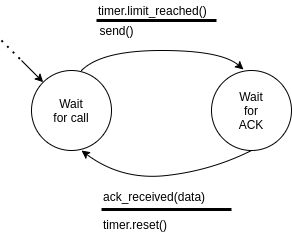
\includegraphics[width=.8\textwidth,height=18em]{img/FSM_Device.png}
\caption{Automa a stati finiti che rappresenta stati e comportamenti di Device}
\label{img:fsm_device}
\end{figure}

\subsection{Classi host: Gateway}

\begin{figure}[H]
\centering{}
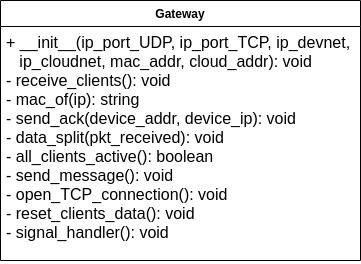
\includegraphics[width=.7\textwidth,height=18em]{img/UML_Gateway.png}
\caption{Schema UML del Gateway}
\label{img:uml_gateway}
\end{figure}

Il \textbf{gateway} viene rappresentato dalla classe Gateway: anch'essa a livello di organizzazione dei metodi ha le stesse caratteristiche della classe \textbf{Device}, come appunto detto nell'apposita sotto-sezione.
%
In questa classe il metodo \emph{receive\_clients()} svolge il ruolo di \emph{main loop}: all'interno di questo ciclo avviene la ricezione del messaggio inviato da uno dei \emph{device}, il messaggio viene poi de-serializzato tramite modulo \textbf{pickle}.
%
Se il messaggio de-serializzato non è un messaggio vuoto \emph{presumiamo} sia quello giusto creando quindi un pacchetto speciale, che è il nostro ACK,  tramite \emph{PacketBuilder}.
Dopodichè il \emph{pacchetto} viene serializzato ed inviato al \emph{device} da cui il \emph{gateway} ha ricevuto l'ultimo pacchetto.

All'interno della classe \textbf{Gateway} c'è una \textbf{struttura dati} molto importante, essenziale per \underline{instradare} i pacchetti dei client nel modo giusto.
%
Si tratta di un \emph{dizionario} dove ogni \underline{chiave} corrisponde ad una \textbf{coppia indirizzo IP, indirizzo MAC} corrispondente ognuna ad un device diverso; ogni \underline{valore} è un riferimento al pacchetto arrivato, può anche non essere arrivato, in questo caso il valore viene impostato a \emph{None}, valore di default.

Dopo questa breve spiegazione della struttura dati utilizzata per la \emph{gestione dei client} passiamo alla fase successiva.
%
Quando un \emph{pacchetto} passa per la data\_split viene verificato se l'indirizzo IP sorgente corrisponde ad uno degli indirizzi IP presenti nella \textbf{arp table modificata}, se la verifica da esito negativo viene sollevata un'\textbf{eccezione}, le socket vengono chiuse e il programma termina perchè vuol dire che ha provato a connettersi un \emph{device non identificato}.
%
Contemporaneamente viene fatto un'altro controllo che analizza il valore di ogni chiave dell'\emph{arp table} e verifica se è nullo.
%
Se queste due condizioni danno esito \emph{positivo}, il \emph{pacchetto} viene inserito nell'\emph{arp table} ed il \textbf{contatore} di clients che hanno inviato il proprio messaggio viene \emph{incrementato}.
%
Nel caso in cui il \textbf{contatore} raggiunge il numero totale di \emph{device} del sistema, quindi 4: viene chiamato il metodo \emph{send\_message()}.

Esso verifica se è già stata aperta una connessione TCP verso il cloud e se non è stato fatto ne apre una:
\begin{figure}[H]
    \centering
    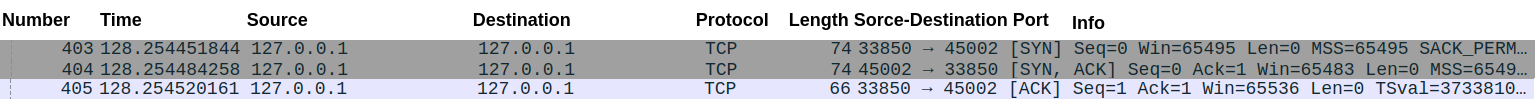
\includegraphics[width=\textwidth,height=25]{img/syncro_TCP.png}
    \caption{Cattura Wireshark: \emph{three-way handshake} \textbf{Gateway} - \textbf{Cloud}}
    \label{fig:syncrotcp}
\end{figure}
Successivamente prende tutti i \textbf{payload} dei pacchetti contenuti nell'\emph{arp table modificata} e li \emph{unisce} in un unico nuovo pacchetto creato tramite \emph{PacketBuilder}, il quale viene poi serializzato ed inviato al \emph{cloud}.
%
Infine tutti i \emph{valori} del dizionario vengono resettati al \emph{valore di default} ed il \emph{contatore} di clients che hanno inviato il proprio messaggio viene \emph{azzerato}.

\begin{figure}[H]
    \centering
    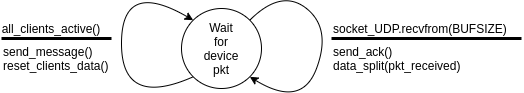
\includegraphics[width=\textwidth,height=7em]{img/FSM_Gateway.png}
    \caption{Automa a stati finiti rappresentante il gateway}
    \label{img:fsm_gateway}
\end{figure}
%
\subsection{Classi host: Cloud}
\begin{figure}[H]
    \centering
    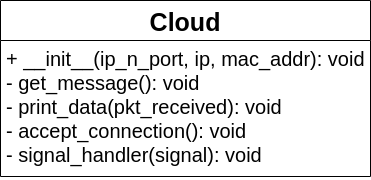
\includegraphics[width=.7\textwidth,height=11em]{img/UML_Cloud.png}
    \caption{Schema UML del Cloud Server}
    \label{img:3}
\end{figure}

Il \emph{Cloud} rappresenta il nostro server cloud TCP, il suo compito è quello di stampare a video le misurazioni ottenute dai dispositivi IoT.
\\
Attraverso il metodo \emph{accept\_connection()} si mette in collegamento con il \emph{Gateway}, di conseguenza aspetta di ricevere il messaggio.
\begin{figure}[H]
    \centering{}
    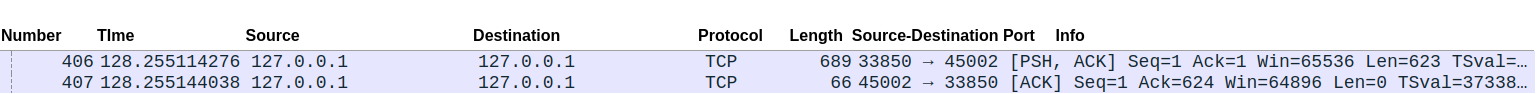
\includegraphics[width=\textwidth,height=25]{img/gateway_send.png}
    \caption{Cattura Wireshark: avvenuta consegna pacchetto ridefinito}
    \label{img:gatewaysend}
\end{figure}
Quando ottiene il pacchetto elaborato, stampa su una console il payload e il tempo di trasmissione.
\begin{figure}[H]
    \centering{}
    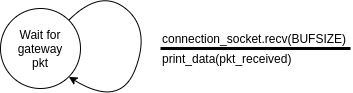
\includegraphics[width=.9\textwidth,height=8em]{img/FSM_Cloud.png}
    \caption{Automa a stati finiti raffigurante il comportamento del Cloud}
    \label{img:fsm_cloud}
\end{figure}

\subsection{Modulo factories}
Nel modulo \textbf{factories} sono presenti 3 classi: \textbf{DeviceFactory, GatewayFactory, CloudFactory}, insieme alle costanti che tengono memoria delle porte UDP e TCP da utilizzare.
%
Tutte e tre condividono lo stesso \emph{pattern} che è il \emph{FactoryMethod}, utile perchè consente di fabbricare oggetti predefiniti che abbiamo poi utilizzato per eseguire la \emph{simulazione} e nella fase di \emph{testing}. Di seguito le varie classi vengono descritte più nel dettaglio.

\begin{figure}[H]
    \centering{}
    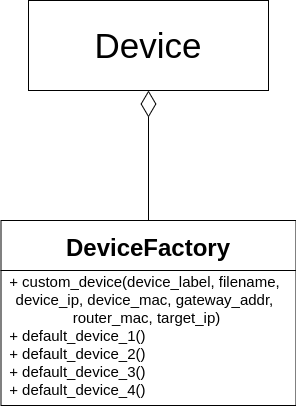
\includegraphics[width=.4\textwidth,height=20em]{img/UML_Device_Factory.png}
    \caption{Diagramma UML della classe DeviceFactory}
    \label{img:uml_devicefactory}
\end{figure}

La classe \emph{DeviceFactory} presenta 5 metodi pubblici: uno che permette la fabbricazione di un device \emph{"custom"}, mentre i restanti 4 fabbricano i \emph{device di default} utili alla \emph{simulazione}.

\begin{figure}[H]
    \centering{}
    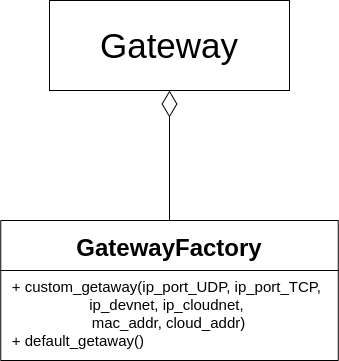
\includegraphics[width=.4\textwidth,height=20em]{img/UML_GatewayFactory.png}
    \caption{Diagramma UML della classe GatewayFactory}
    \label{img:uml_gatewayfactory}
\end{figure}

La classe GatewayFactory fornisce due metodi pubblici: uno per produrre gateway a piacimento e l'altro per generare il \emph{gateway di default} utile alla \emph{simulazione}.

\begin{figure}[H]
    \centering{}
    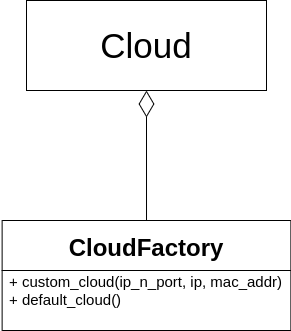
\includegraphics[width=.4\textwidth,height=20em]{img/UML_CloudFactory.png}
    \caption{Diagramma UML della classe GatewayFactory}
    \label{img:uml_cloudfactory}
\end{figure}

La classe CloudFactory contiene due metodi pubblici anch'essa: uno sempre per la fabbricazione di oggetti \emph{custom} e l'altro per la creazione del \emph{server cloud} utile alla \emph{simulazione}.

\subsection{Note sui buffer utilizzati nei vari canali}
I \emph{canali} utilizzati per la comunicazione fra i vari host sono 2 per \emph{device}: uno per l'inoltro delle misurazioni al \emph{gateway} il quale poi apre il canale con lo stesso dispositivo per inviare l'\emph{ACK}.
%
Vi è poi un altro collegamento via \emph{TCP} tra gateway e cloud.

Per quanto riguarda il \textbf{buffer} di ogni device, utilizzato per ricevere gli ACK che sono messaggi di dimensione inferiore ai 400 byte, ci è sembrato opportuno impostarli a 1024 byte in modo da non creare un \emph{overhead}.

Vale lo stesso per il \textbf{buffer} del \emph{gateway}, dedicato alla \underline{ricezione dei pacchetti} dei client, in quanto questi ultimi non superano di norma i 500 byte.

Infine, il \textbf{buffer} del \emph{cloud} è quello con dimensione maggiore(4096 byte) perchè il \emph{gateway} prima di inviare il pacchetto lo riempie con il payload dei 4 pacchetti arrivati dai device, per cui risulterà più pesante.

Siccome vengono sommati soltanto i \emph{payload}, il Packet risultante non sarà il quadruplo. Nonostante ciò, come osservato nelle \textbf{catture di Wireshark} eseguite durante il testing dell'applicativo, il pacchetto si mostra comunque più grande di 1024 Byte per questo è necessario un \emph{buffer più grosso}.
\newline
\newline
\textbf{Nota Bene:} Le seguenti considerazioni sono valide soltanto per invii periodici dove il periodo è uguale a 60 secondi, come nella nostra simulazione.
\chapter{Sviluppo}
\section{Testing}
Dopo aver descritto la struttura del software, andiamo ad analizzare una componente fondamentale del progetto, ovvero il \textbf{testing} del programma.
Purtroppo, non avendo a disposizione un ambiente per fare testing automatizzato, abbiamo optato per vie più manuali.
\\
Attraverso la creazione di alcuni \textbf{script di test} tutti contenuti nella cartella omonima:
\begin{itemize}
    \item \emph{test\_dev1.py}: mette in esecuzione il \emph{device IoT} con IP: 192.168.1.10
    \item \emph{test\_dev2.py}: mette in esecuzione il \emph{device IoT} con IP: 192.168.1.15
    \item \emph{test\_dev3.py}: mette in esecuzione il \emph{device IoT} con IP: 192.168.1.20
    \item \emph{test\_dev4.py}: mette in esecuzione il \emph{device IoT} con IP:
    192.168.1.25
    \item \emph{test\_devices.py}: mette in esecuzione tutti e 4 i device, sfruttando il modulo \textbf{subprocess}
    \item \emph{test\_gateway.py}: mette in esecuzione il \emph{gateway}
    \item \emph{test\_cloud.py}: mette in esecuzione il \emph{cloud}
\end{itemize}

I soprastanti script vengono utilizzati anche per la simulazione, devono essere eseguiti nel seguente ordine per funzionare correttamente: 
\begin{itemize}
    \item test\_cloud.py \textgreater test\_gateway.py \textgreater test\_devices.py
    \item test\_cloud.py \textgreater test\_gateway.py \textgreater test\_dev1.py \textgreater test\_dev2.py \textgreater test\_dev3.py \textgreater test\_dev4.py 
\end{itemize}

\section{Metodologia di lavoro}

Durante tutte le fasi del progetto abbiamo lavorato in coppia da \textbf{remoto} o in \textbf{presenza} coordinandoci nelle diverse operazioni da svolgere.
%
Per la maggior parte del tempo abbiamo lavorato in coppia mentre per la relazione ci siamo divisi i vari paragrafi per poi integrarli alla fine.
%
Inoltre per la fase di programmazione vera e propria ed anche per la stesura di questa relazione ci siamo concentrati insieme su ogni singolo problema.

\section{Note di sviluppo}

Il \emph{linguaggio di programmazione} utilizzato per lo sviluppo del progetto è \textbf{Python}.
\\
Sono stati utilizzati dei moduli non studiati in laboratorio: 
\begin{itemize}
    \item il modulo \textbf{pickle} che grazie ai metodi \emph{dumps(data)} e \emph{loads(data)} permette di serializzare/deserializzare oggetti;
    \item il modulo \textbf{subprocess} che permette di eseguire più sotto-programmi all'interno di un singolo programma.
\end{itemize}

\appendix
\chapter{Guida utente}

Per l'avvio del programma seguire le seguenti istruzioni:
\begin{enumerate}
    \item Lanciare il cloud in una console specializzata con il comando:
    \begin{itemize}
        \item python test\_cloud.py
    \end{itemize}
    \item Lanciare il gateway in una console specializzata con il comando:
    \begin{itemize}
        \item python test\_gateway.py
    \end{itemize} 
    \item Lanciare i 4 dispositivi in una console specializzata con il comando:
    \begin{itemize}
        \item python test\_devices.py
    \end{itemize} 
    \item O in alternativa lanciare i 4 device su console differenti:
    \begin{itemize}
        \item python test\_dev1.py
        \item python test\_dev2.py
        \item python test\_dev3.py
        \item python test\_dev4.py
    \end{itemize}
\end{enumerate}

\textbf{N.B.} Prima di eseguire le istruzioni, controllare di essere posizionati sulla cartella 'test'.
%
\newline
\newline
Premere \textbf{Ctrl+C} su ogni console avviata per interrompere il programma.
\end{document}